\documentclass[a4paper, 12pt]{report}

\usepackage[utf8]{inputenc} 	% accents
\usepackage[T1]{fontenc}      	% caractères français
\usepackage{graphicx}		% images
\usepackage{listings}		% Affichage code source
\usepackage{amsmath}

\lstset{ % Permet d'utiliser des accents dans lstlisting
     literate=%
         {á}{{\'a}}1
         {é}{{\'e}}1
         {è}{{\`e}}1
}

\title{Projet INFO-H-303 : Villo!}
\author{Hereman Nicolas, Van Brande Rodrigue}
\date{24 avril 2015}

\begin{document}
\maketitle 

\section*{Diagramme entité-association} % Diagramme
	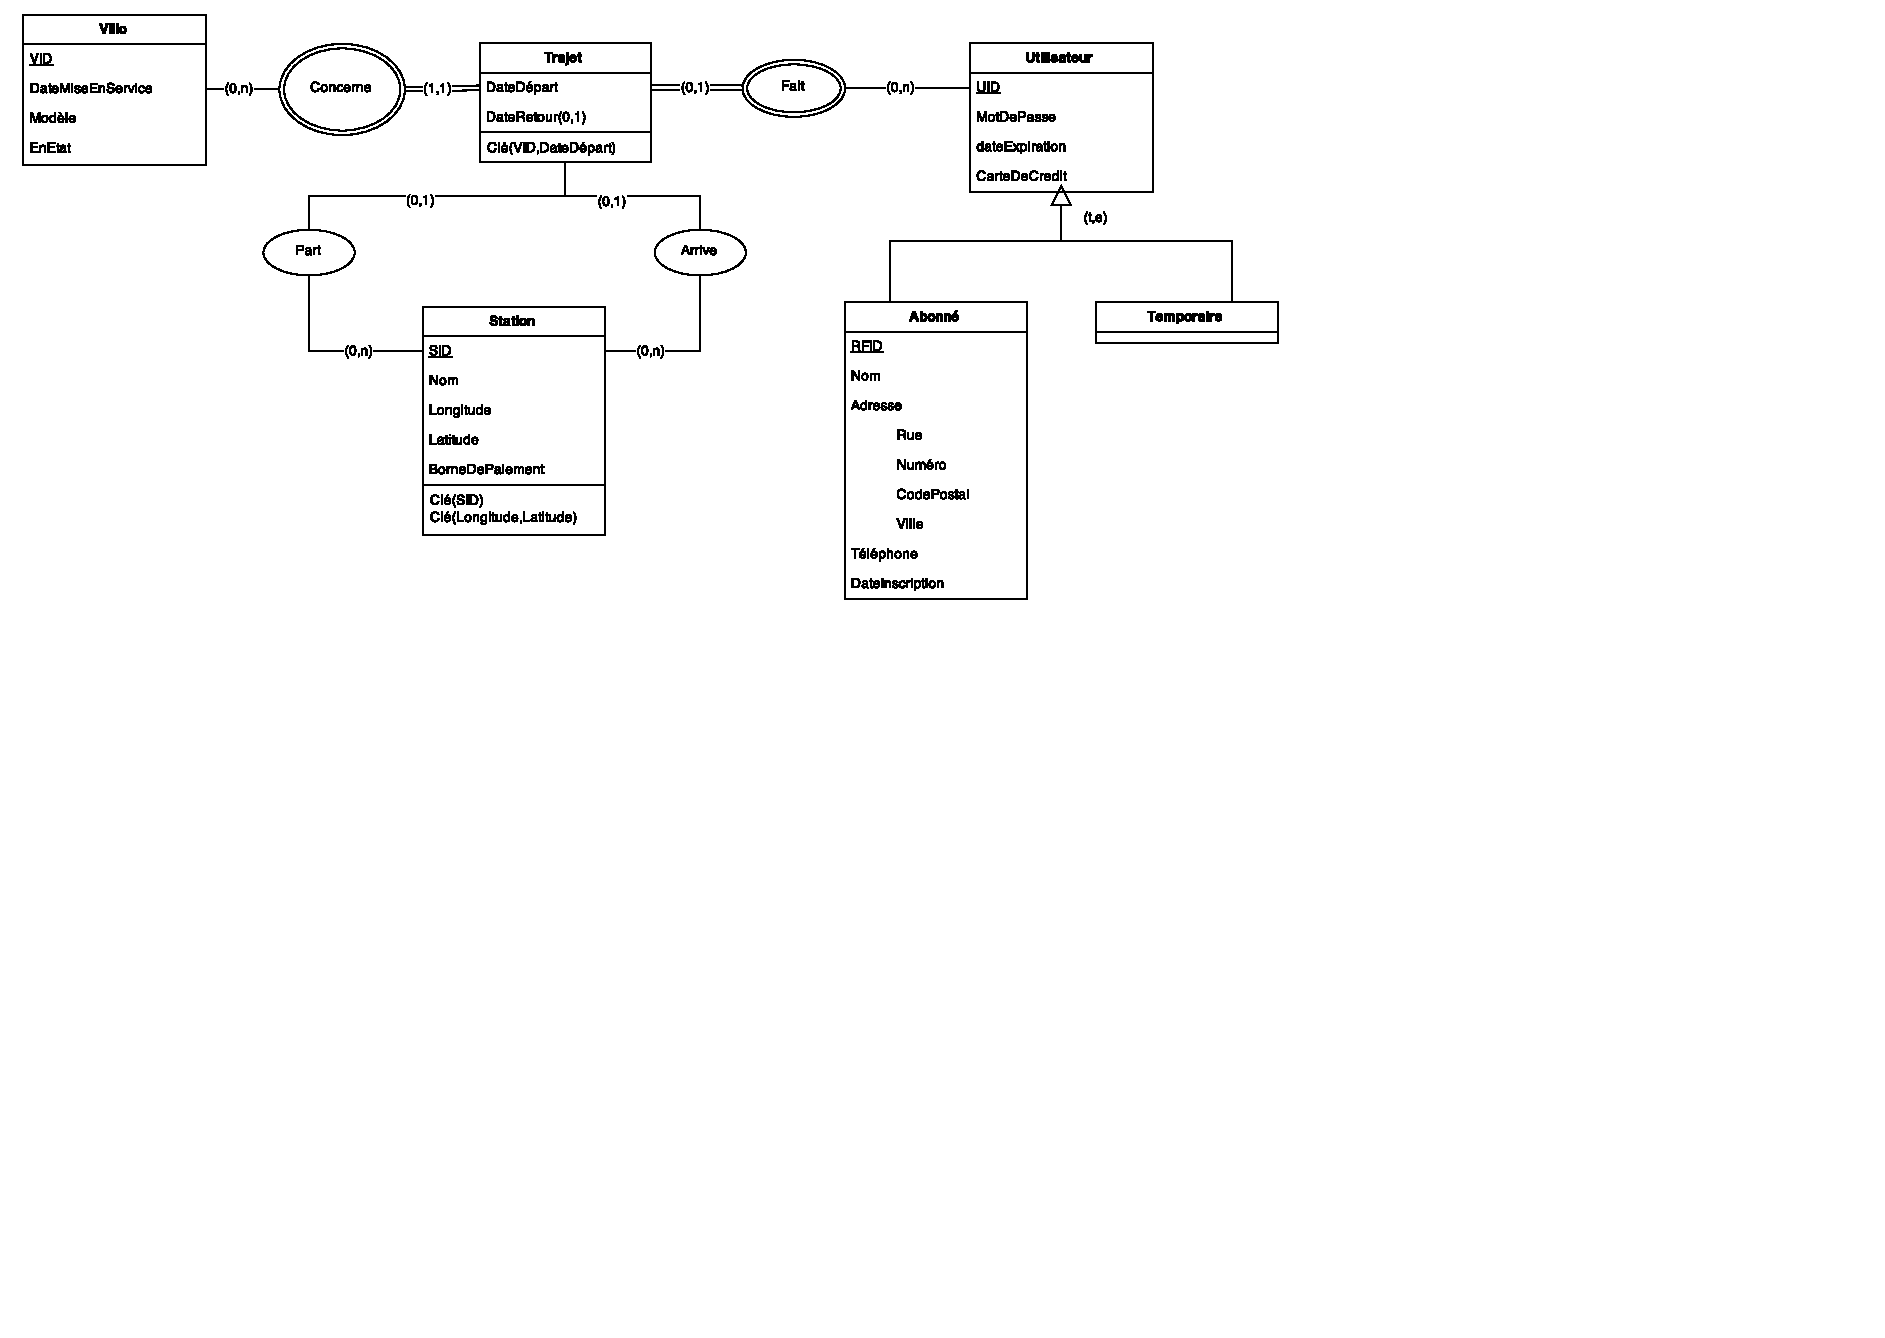
\includegraphics[scale=0.8]{entityassocdiagram.pdf}

\section*{Contraintes et hypothèses} %Contraintes

	\begin{itemize}
		\item La \textit{DateExpiration} d'un \textit{Abonné} doit être strictement supérieure à sa \textit{DateInscription}
		
		\item La \textit{DateDépart} d'un \textit{Trajet} doit être strictement supérieure à la \textit{DateInscription} de l'\textit{Abonné} qui le fait.
		
		\item La \textit{DateDépart} d'un \textit{Trajet} pot être strictement inférieure à la \textit{DateExpiration} de l'\textit{Utilisateur}.
		
		\item La \textit{DateDépart} d'un \textit{Trajet} doit être strictement inférieure à la \textit{DateExpiration} de l'\textit{Utilisateur} qui le fait.
		
		\item La \textit{DateRetour} d'un \textit{Trajet} doit être strictement supérieure à la \textit{DateDépart} de ce même \textit{Trajet}.
		
		\item La \textit{DateDépart} d'un \textit{Trajet} doit être strictement supérieure à la \textit{DateMiseEnService} du \textit{Villo} concerné.
		
		\item A l'instant \textit{DateRetour}, la \textit{Station} de retour d'un \textit{Trajet} doit contenir moins de \textit{Villos} que sa \textit{Capacité}. Le calcul du nombre de \textit{Villos} présents dans une \textit{Station} à l'aide de l'entité \textit{Trajet}.
		
		\item Un même \textit{Villo} ne peut pas concerner deux \textit{Trajets} en même temps.
		
		\item Un même \textit{Utilisateur} ne peut pas faire deux \textit{Trajets} en même temps.
		
		\item Un \textit{Trajet i} qui suit directement un autre \textit{Trajet j} pour un même \textit{Villo} doit avoir la même \textit{Station} de départ que la \textit{Station} d'arrivée du \textit{Trajet j}.
		
		\item Si un \textit{Trajet} n'a pas d'\textit{Utilisateur}, il n'a pas de \textit{Station} de départ et inversement.
		
		\item Si un \textit{Trajet} n'a ni \textit{Utilisateur} ni \textit{Station} de départ, sa \textit{DateDépart} est 0000/00/00 - 00:00:00
		
		\item Pour chaque \textit{Villo}, il n'y a qu'un \textit{Trajet} sans \textit{Utilisateur} et \textit{Station} de départ. Ni plus ni moins.
		\item Si un \textit{Trajet} n'a pas de \textit{Station} de retour, il n'a pas de \textit{DateRetour} et inversement.
		
		\item Pour chaque \textit{Villo},  il y a au maximum un \textit{Trajet} sans \textit{DateRetour} et \textit{Station} de retour.
		
		\item Si un \textit{Trajet} n'a pas de \textit{DateDépart}, il a une \textit{DateRetour}.
		
		\item Si un \textit{Trajet} n'a pas de \textit{DateRetour}, il a une \textit{DateDépart}.
		
	\end{itemize}

\section*{Traduction relationnelle} %Relation
	
	\begin{itemize}
	
		\item Utilisateur(\underline{UID},MotDePasse,DateExpiration,CarteDeCredit)
		
		\item Abonne( \underline{UID}, \underline{RFID}, Nom, Rue, Numéro, CodePostal, Ville, Téléphone, DateInscription)
		
		\begin{itemize}
			\item UID référence Utilisateur.UID
		\end{itemize}
		
		\item Station(\underline{SID}, Nom, \underline{Longitude, Latitude}, Capacité, BorneDePaiement)
		
		\item Villo(\underline{VID},DateMiseEnService,Modèle, EnEtat)
		
		\item Trajet(\underline{VID,DateDépart}, \textit{UID}, \textit{StationDépart}, \textit{DateRetour}, \textit{StationRetour})
		
		\begin{itemize}
			\item UID référence Utilisateur.UID
			\item VID référence Villo.VID
			\item StationDépart référence Station.SID
			\item StationRetour référence Station.SID
		\end{itemize}
		
	\end{itemize}
	
	\subsection*{Remarque}
	Un Utilisateur.UID n'existant pas dans Abonné.UID est un utilisateur temporaire

\section*{Justification et hypothèses de modélisation} % Justification

On utilise une table \textit{Utilisateur} pour stocker leurs données. On a créé une table \textit{Abonné} afin des les différencier des utilisateurs \textit{Temporaire}. Comme l'héritage des table est totale et exclusive et que toutes les informations dont on a besoin pour ces derniers sont déjà dans la table \textit{Utilisateur}, ils n'ont pas besoin d'une table pour eux. Les utilisateurs temporaires seront ceux qui n'ont pas leurs \textit{UID} dans la table \textit{Abonné}.

Les \textit{Stations} et \textit{Villos} ont aussi droit à leur table pour qu'on y sauvegarde leurs données.

On sauvegarde aussi la liste des \textit{Trajets} dans une table. Le fait que l'\textit{Utilisateur} et la \textit{StationDépart} soit optionnel peut paraître illogique par rapport à la réalité. Mais cela se justifie par le fait que les \textit{Villo} doivent être placé une première fois. Comme on ne sauvegarde pas la \textit{Station} dans laquelle ils sont stockés, on se repère au \textit{Trajet} pour le savoir. On les place donc à l'aide de \textit{Trajet} sans \textit{Station} de départ et sans \textit{Utilisateur}. Les \textit{Trajets} sans \textit{Station} de retour et \textit{DateRetour} sont les \textit{Trajets} encore en cours.

\section*{Script SQL DDL de création de base de données}

\lstset {numbers=left ,numberstyle=\tiny \bfseries \underline , stepnumber=1,firstnumber=1,numberfirstline=true}

\begin{lstlisting}[language=sql]
CREATE TABLE `Utilisateur` (
	`UID` int unsigned NOT NULL,
	`MotDePasse` smallint(4) unsigned zerofill NOT NULL,
	`CarteDeCredit` bigint(16) unsigned zerofill NOT NULL,
	`DateExpiration` datetime NOT NULL,
	PRIMARY KEY (`UID`)
);

CREATE TABLE `Villo` (
	`VID` smallint unsigned NOT NULL,
	`DateMiseEnService` datetime NOT NULL,
	`Modèle` varchar(12) NOT NULL,
	`EnEtat` tinyint(1) NOT NULL,
	PRIMARY KEY (`VID`)
);

CREATE TABLE `Abonné` (
	`UID` int unsigned NOT NULL,
	`RFID` char(20) NOT NULL,
	`Nom` varchar(50) NOT NULL,
	`Rue` varchar(100) NOT NULL,
	`Numéro` smallint unsigned NOT NULL,
	`CodePostal` smallint(4) unsigned NOT NULL,
	`Ville` varchar(50) NOT NULL,
	`Téléphone` char(10) NOT NULL,
	`DateInscription` datetime NOT NULL,
	PRIMARY KEY (`RFID`),
	FOREIGN KEY (`UID`) REFERENCES Utilisateur(`UID`)
);

CREATE TABLE `Station` (
	`SID` smallint unsigned NOT NULL,
	`Nom` varchar(50) NOT NULL,
	`Longitude` float NOT NULL,
	`Latitude` float NOT NULL,
	`Capacité` tinyint unsigned NOT NULL,
	`BorneDePaiement` tinyint(1) NOT NULL,
	PRIMARY KEY (`SID`,`Longitude`,`Latitude`)
);

CREATE TABLE `Trajet` (
	`VID` smallint unsigned NOT NULL,
	`DateDépart` datetime NOT NULL DEFAULT '0000-00-00 00:00:00',
	`UID` int unsigned DEFAULT NULL,
	`StationDépart` smallint unsigned DEFAULT NULL,
	`DateRetour` datetime DEFAULT NULL,
	`StationRetour` smallint unsigned DEFAULT NULL,
	PRIMARY KEY (`VID`,`DateDépart`),
	FOREIGN KEY (`VID`) REFERENCES Villo(`VID`),
	FOREIGN KEY (`UID`) REFERENCES Utilisateur(`UID`),
	FOREIGN KEY (`StationDépart`) REFERENCES Station(`SID`),
	FOREIGN KEY (`StationRetour`) REFERENCES Station(`SID`)
);
\end{lstlisting}

\section*{Les requêtes en algèbre relationnel et calcul relationnel tuples} %Requêtes

\subsection*{R1}

Les utilisateurs habitant Ixelles ayant utilisé un Villo de la station Flagey

\subsubsection*{Algèbre relationnelle}

$UTS\leftarrow (Abonne * Trajet)\bowtie_{StationDepart=SID} Station$

$Sel\leftarrow \sigma_{Nom=Flagey\wedge Ville=Ixelles}(UTS)$

$\pi_{UID}(Sel)$

\subsubsection*{Calcul relationnel tuple}

\begin{multline*}
\{  a.UID | Abonne(a)\wedge a.Ville='Ixelles' \wedge \exists t \exists s ( Trajet(t)\wedge Station(s) \\\wedge t.UID=a.UID \wedge s.Nom='Flagey')   \} 
\end{multline*}

\subsubsection*{SQL}
\begin{lstlisting}[language=sql]
SELECT a.UID FROM Trajet t, Abonné a, Station s 
WHERE a.UID=t.UID AND s.SID=t.StationDépart
AND a.Ville="Ixelles" AND s.Nom="Flagey"
\end{lstlisting}

\subsubsection*{Imprécisions}

L'énoncé ne dit pas si il faut récupérer l'UID où le nom de l'utilisateur. Nous avons donc supposé qu'il s'agissait de l'UID.

\subsection*{R2}

Les utilisateurs ayant utilisé Villo au moins 2 fois
\subsubsection*{Algèbre relationnelle}

$T(u,v,d) \leftarrow\pi_{UID,VID,DateDepart}(Trajet)$

$Temp\leftarrow Trajet\bowtie_{UID=u}T $

$\pi_{UID}( \sigma_{VID\neq v\vee DateDepart\neq d}(Temp)  )$

\subsubsection*{Calcul relationnel tuple}

\begin{multline*}
\{ u.UID|Utilisateur(u)\wedge\exists t1\exists t2 ( Trajet(t1)\wedge Trajet(t2)\wedge t1.UID=u.UID\wedge \\
t2.UID=u.UID \wedge [t1.VID\neq t2.VID\vee t1.DateDepart\neq t2.DateDepart] )  \}
\end{multline*}

\subsubsection*{SQL}
\begin{lstlisting}[language=sql]
SELECT t1.UID FROM Trajet t1, Trajet t2 WHERE t1.UID=t2.UID
AND ( t1.DateDépart!=t2.DateDépart OR t1.VID!=t2.VID ) 
GROUP BY t1.UID
\end{lstlisting}

\subsubsection*{Imprécisions}

Voir \textit{R1}.

\subsection*{R3}

Les paires d'utilisateurs ayant fait un trajet identique
\subsubsection*{Algèbre relationnelle}

$t2(UID2,dep2,ret2)\leftarrow\pi_{UID,StationDepart,StationRetour}(Trajet)$

$Temp\leftarrow Trajet\bowtie_{StationDepart=dep2\wedge StationRetour=ret2}t2$

$\pi_{UID,UID2}(\sigma_{UID\neq UID2} Temp)$

\subsubsection*{Calcul relationnel tuple}

\begin{multline*}
\{  u1.UID, u2.UID |Utilisateur(u1)\wedge Utilisateur(u2)\wedge u1.UID \neq u2.UID\wedge \\
\exists t1\exists t2 ( Trajet(t1)\wedge Trajet(t2) \wedge
 t1.UID=u1.UID \wedge t2.UID=u2.UID \wedge \\
  t1.StationDepart=t2.StationDepart \wedge t1.StationRetour=t2.StationRetour )  \}
\end{multline*}

\subsubsection*{SQL}
\begin{lstlisting}[language=sql]
SELECT t1.UID, t2.UID FROM Trajet t1, Trajet t2
WHERE t1.StationDépart=t2.StationDépart
AND t1.StationRetour=t2.StationRetour
AND t1.UID!=t2.UID
GROUP BY t1.UID,t2.UID
\end{lstlisting}

\subsubsection*{Imprécisions}

Voir \textit{R1}.

\subsection*{R4}

Les vélos ayant deux trajets consécutifs disjoints ( station de retour du premier trajet différente de la station de départ du suivant).
\subsubsection*{Algèbre relationnelle}

TODO % TODO

\subsubsection*{Calcul relationnel tuple}

TODO % TODO

\subsubsection*{SQL}
TODO%TODO

\subsubsection*{Imprécisions}

TODO%TODO

\subsection*{R5}

Les utilisateurs, la date d'inscription, le nombre total de trajet effectués, la distance totale parcourue et la distance moyenne parcourue par trajet, classés en fonction de la distance totale parcourue.

\subsubsection*{SQL}

\begin{lstlisting}[language=sql]
SELECT t1.uid, a.DateInscription, t1.nb, di.dist, di.adist 
FROM 
(SELECT Trajet.UID, t.nb FROM Trajet
	INNER JOIN
	(SELECT tr.UID as uid, COUNT(*) as nb FROM Trajet 
			as tr GROUP BY tr.UID ) as t
	ON Trajet.UID = t.uid
	GROUP BY t.uid ) as t1,
Abonné a,
(SELECT tra.UID as uid, 
	SUM( SQRT(POW(s2.Longitude-s1.Longitude,2) +
	 	POW(s2.Latitude-s1.Latitude,2)) ) as dist,
	AVG( SQRT(POW(s2.Longitude-s1.Longitude,2) + 
		POW(s2.Latitude-s1.Latitude,2)) ) as adist
	FROM Trajet tra, Station s1, Station s2
	WHERE tra.StationDépart = s1.SID
	AND tra.StationRetour = s2.SID
	GROUP BY tra.UID) as di
WHERE t1.uid = a.UID
AND di.uid = a.UID
ORDER BY di.dist
\end{lstlisting}

\subsubsection*{Imprécisions}

Comme pour \textit{R1}, on a décidé d'utiliser l'\textit{UID} plutôt que le \textit{Nom} de l'\textit{Utilisateur}.
Pour les distances, il n'est pas précisé d'unité. Nous avons donc pris la décision d'utiliser directement les coordonnées géographiques ( Longitude et Latitude ) sans aucune conversion pour les calculer.
\subsection*{R6}

Les stations avec le nombre total de vélos déposés dans cette station ( un même vélo peut-être comptabilisé plusieurs fois) et le nombre d'utilisateurs différent ayant utilisé la station et ce pour toutes les stations ayant été utilisées au moins 10 fois.

\subsubsection*{SQL}
TODO%TODO

\end{document}
% FIN DU DOCUMENT